\chapter{Model physics}\label{chap:model_physics}

\section{How to navigate this chapter}
One should navigate this chapter in the following manner: Start here and read from left to right. In about 20 minutes you will reach the end of this chapter, where you can jump to Chapter three. In Chapter three, our discretization experts will BLOW YOUR MIND with some top class numerical jargon. However, please do not let excitement get the better of you. Read this chapter first as it took two Welshmen an awful lot of time to write it, cull it and then write it again. The material covered in this chapter is dealt with in great detail in \citet{batchelor1967} and \citet{landau}. \cite{cushman1994,panton2006,vallis2006,gill1982} are also useful references.

\section{Advection--Diffusion Equation}\label{Sect:MP-AdvdifEqn}

\subsection{Derivation \& Equations}

The general form the equation that governs the evolution of a scalar field $c$
(\eg passive tracer, species concentration, temperature, salinity) is
\begin{equation}\label{eq:general_scalar_eqn}
\ppt{c} + \nabla\cdot(\bmu c) = \nabla\cdot(\kaptens\nabla c) - \sigma c + F,
\end{equation}
where $\bmu=(u,v,w)$ is the velocity vector, $\kaptens$ is the diffusivity, $\sigma$ is an absorption term and $F$ represents any source or reaction terms.

\subsubsection{Advection}
The advection term in \eqref{eq:general_scalar_eqn}, given by
\begin{equation}\label{eq:scalar_advection}
\nabla\cdot(\bmu c) = \bmu\cdot\nabla c + (\nabla\cdot\bmu)c,
\end{equation}
expresses the transport of the scalar quantity $c$ in the flow field $\bmu$. Note that for an incompressible flow $\nabla\cdot\bmu=0$ resulting in the second term on the right hand side of \eqref{eq:scalar_advection} dropping out. However, there may be numerical
reasons why the discrete velocity field is not exactly divergence free, in which case this term may
be included in the discretisation (see section \ref{Sect:ND_advection_diffusion_discretisation}). Note also that the second term on
the \rhs\ of \eqref{eq:scalar_advection} may be interpreted as a source term for $c$.When this motion is largely in the vertical direction resulting from temperature (density) differences the term convection is often used to describe this.

\subsubsection{Diffusion}
The diffusion term in \eqref{eq:general_scalar_eqn}, given by 
\begin{equation}\label{eq:scalar_diffusion}
\nabla\cdot(\kaptens\nabla c),
\end{equation}
represents the mixing of $c$ and may be due to 
molecular mixing of individual particles via Brownian motion, or mixing via large (in comparison to the
molecular scale) eddies in the flow. For many applications \eqref{eq:scalar_diffusion} can be written in a simpler form. Often, diffusion is isotropic giving $\kaptens = \mathrm{diag}(\kappa,\kappa,\kappa)$ and thus the diffusion term
may be written as
\begin{equation}\label{eq:scalar_isotropic_diffusion}
\nabla\cdot(\kaptens\nabla c) = \kappa\nabla\cdot\nabla c = \kappa\nabla^2 c = \kappa\Delta c.
\end{equation}
In domains with high aspect ratio dynamics one often uses a smaller value of diffusivity in the `thin'
direction. For example, in the atmosphere or ocean we may choose a horizontal diffusivity $\kappa_H$ and a
vertical diffusivity $\kappa_V$ so that $\kaptens = \mathrm{diag}(\kappa_H,\kappa_H,\kappa_V)$ with $\kappa_V < \kappa_H$.
In this case the diffusion term may be written as
\begin{equation}\label{eq:scalar_isotropic_diffusion}
\nabla\cdot(\kaptens\nabla c) = \kappa_H \left(\pptt[x]{c} + \pptt[y]{c}\right) + \kappa_V \pptt[z]{c}.
\end{equation}
Note that this second order term is often termed Laplacian diffusion. The corresponding 4th order version is sometimes
termed hyper-diffusion and acts in a similar manner to Laplacian diffusion but is more
scale selective.

\subsection{Boundary Conditions} \label{Sect:BCs}

\index{boundary conditions}

To form a well-posed system upon which to attempt a numerical discretisation, the
set of equations (discussed above) describing the behaiour of the 
system must be supplemented with appropriate boundary conditions.


\subsubsection{Dirichlet condition for a scalar field}\label{sect:bc_scalar_dirichlet}
\index{boundary conditions!Dirichlet}
For a scalar field, $T$ say, a Dirichlet condition on the boundary
$\partial\Omega$ takes the form
\begin{equation*}
T=\tilde{T},\quad \textrm{on}\quad \partial\Omega.
\end{equation*}


\subsubsection{Neumann condition for a scalar field}\label{sect:bc_scalar_neumann}
\index{boundary conditions!Neumann}
\index{advection-diffusion equation}
Taking the weak form (applying Green's theorem to the diffusion term) of the advection-diffusion equation \eqref{eq:general_scalar_eqn} leads to a surface integral of the form
\begin{equation*}
\int_{\partial\Omega} N_i (\kaptens\nabla T)\cdot\bmn \;d\Gamma.
\end{equation*}
The Neumann condition is specified by assigning a value to $(\kaptens\nabla T)\cdot\bmn$, \eg
\begin{equation*}
(\kaptens\nabla T)\cdot\bmn = q,\quad \textrm{on}\quad \partial\Omega,
\end{equation*}
and adding in this surface integral to the discretised equation.


\subsubsection{Robin condition for a scalar field}\label{sect:bc_scalar_robin}
\index{boundary conditions!Robin}
The Robin condition is similar to the Neumann condition but instead takes the form
\begin{equation*}
(\kaptens\nabla T)\cdot\bmn + \alpha T = q,\quad \textrm{on}\quad \partial\Omega.
\end{equation*}


\subsubsection{Prescribed Dirichlet condition for momentum --- no-slip as a special case}\label{sect:bc_vector_dirichlet}
\index{boundary conditions!Dirichlet}
\index{momentum equation}
This condition for momentum is set by simply prescribing all three components of
velocity. For example, we might specify an inflow boundary where the normal component
of velocity is non-zero, but the two tangential directions are zero. A special case is
where all three components are zero and this is referred to as no-slip.


\subsubsection{Prescribed stress condition for momentum --- free-stress as a special case}\label{sect:bc_scalar_stress}
\index{boundary conditions!prescribed stress}
\index{traction force}
\index{momentum equation}
As for the scalar equation, applying Green's theorem to the stress term and the pressure
gradient in \eqref{mtm} results in a surface integral of the form
\begin{equation}\label{StressBC}
\tautens\cdot\bmn - p\bmn = \bmF,\quad \textrm{on}\quad \partial\Omega,
\end{equation}
where $\bmF$ is an applied 'traction' force (actually a force per unit area or stress, it becomes
a force when the surface integral in the weak form is performed). An example of this might be were we set the vertical
component to zero (in the presence of a free surface) and impose the two tangential directions
(\eg a wind stress).

\index{boundary conditions!free stress}
The free-stress condition
is the case where we take $\bmF\equiv\vec{0}$.


\subsubsection{Traction boundary condition for momentum --- free-stress as a special case}\label{sect:bc_scalar_traction}
\index{boundary conditions!traction}
\index{momentum equation}
In this case the normal component of velocity can be prescribed (\eg inflow or
no-flow ($g=0$) through the boundary)
\begin{equation*}
\bmu\cdot\bmn = g,\quad \textrm{on}\quad \partial\Omega.
\end{equation*}
The remaining two degrees of freedom are imposed by taking the
tangential component of \eqref{StressBC} and specifying the tangential component
of the force $\bmF_{\tau}$, \ie
\begin{equation*}
\bmtau\cdot(\tautens\cdot\bmn - p\bmn) = \bmtau\cdot\tautens\cdot\bmn = \bmF_{\tau},\quad \textrm{on}\quad \partial\Omega,
\end{equation*}
An example of this might be where a rigid lid is used (so normal component is zero)
and the tangential components are a prescribed wind stress (in which case we take
the two tangential directions to correspond to the available stress or wind velocity
information, \ie east-west and north-south) or bottom drag. Also, what we often term free-slip
where the tangential components of stress are set to zero.

Apologies for the bad notation, $\tau$ here is the tangential direction
vectors (two of them) and $\tautens$ is the viscous stress tensor.

\section{Momentum Equations}\label{Sect:MP-MomEqn}

\subsection{Derivation \& Equations}

The state of a moving fluid can be described mathematically through means of
functions which give the distribution of velocity $\bmu=\bmu(\bmx,t)$ and
any two thermodynamics quantities (such as the pressure $p(\bmx,t)$ and
density $\rho(\bmx,t)$) within the fluid. All thermodynamic quantities are
determined by the values of any two such quantities together with the
equation of state. \citet{batchelor1967} is the ultimate reference to much of this
material. However, \cite{landau,cushman1994,panton2006,vallis2006,gill1982} are also
useful. \fluidity\ can solve the equations of motion in varying forms, and
with various approximations. These forms and approximations are discussed in
the following sections.

\index{conservation!equation}
\index{momentum equation}

A starting point for describing the physics of a continuum are the conservation equations. Fluid volumes deform in time as the fluid moves. If $\theta(\bmx,t)$ is the density of some quantity (\eg Temperature) associated with the fluid, the time evolution of that quantity in a fluid volume $V(t)$ is 
\begin{equation}\label{RTT}
 \ddt{}\left[\int_{V(t)}\theta(\bmx,t)\right]=
 \int_{V(t)}\left(\DDt{\theta}+\theta\nabla\cdot\bmu\right),
\end{equation}
\index{Reynolds Transport theorem}
which is the Reynolds' Transport theorem. In \eqref{RTT} $\bmx=(x,y,z)^T$ and $\bmu=(u,v,w)^T$ are three dimensional position and velocity vectors respectively and 
\begin{equation}\label{MatDiv}
 \DDt{}\equiv\frac{\partial}{\partial{t}}+\bmu\cdot\nabla,
\end{equation}
is the \textit{material derivative}.

\subsubsection{Mass conservation}
\index{conservation!mass}
Since matter is neither created nor destroyed, substituting $\theta=\rho$ in \eqref{RTT} gives that the \lhs\ is zero. Then, as the volume $V(t)$ is arbitrary, it is seen that the mass density satisfies
\begin{equation}\label{mass_conservation}
 \DDt{\rho}=-\rho\nabla\cdot\bmu,
\end{equation}
or equivalently
\begin{equation}\label{mass_conservation_2}
 \frac{\partial\rho}{\partial{t}}+\nabla\cdot(\rho\bmu)=0.
\end{equation}
The quantity $\rho\bmu$ is called the \textit{mass flux} or \textit{momentum} and \eqref{mass_conservation_2} is termed the \textit{equation of continuity}.

\subsubsection{Momentum conservation}
\index{conservation!momentum}
The momentum associated with a unit volume of fluid is given by $\rho\bmu$. Initially, the fluid will be considered \textit{ideal}, that is, viscosity and conductivity are assumed to be unimportant. Then, the rate of change of momentum is given by
\begin{equation}\label{mom_cons_1}
 \frac{\partial}{\partial{t}}(\rho\bmu)=\rho\frac{\partial\bmu}{\partial{t}}+\frac{\partial\rho}{\partial{t}}\bmu.
\end{equation}
Using the equation of continuity \eqref{mass_conservation_2} and Euler's
equation \citep{batchelor1967}, which is the force equation for an inviscid fluid, in the form
\begin{equation}\label{mom_cons_2}
 \frac{\partial\bmu}{\partial{t}}=-\bmu\cdot\nabla\bmu-\frac{1}{\rho}\nabla{p},
\end{equation}
gives
\begin{equation}\label{mom_cons_3}
 \frac{\partial}{\partial{t}}(\rho\bmu)=-\nabla{p}-\nabla\cdot(\rho\bmu\bmu),
\end{equation}
where $\bmu\bmu$ is a tensor which represents the dyadic product of vectors which can be written $[\bmu\bmu]_{ij}=u_{i}u_{j}$. Writing $\tensor{\Pi}=p\mathbf{I}+\rho\bmu\bmu$ \eqref{mom_cons_3} can finally be written as
\begin{equation}\label{mom_cons_4}
 \frac{\partial}{\partial{t}}(\rho\bmu)+\nabla\cdot\tensor{\Pi}=0,
\end{equation}
where $\tensor{\Pi}$ is clearly a symmetric tensor and is termed the \textit{momentum flux density tensor}.

\subsection{Approximations}

\subsubsection{Incompressibility} \label{sect:incompressibility}
A number of assumptions lead to the consideration of an incompressible fluid or flow (see section \ref{sect:equation_of_state}). In this case one replaces the continuity equation \eqref{nonconmass} with:
\begin{equation}\label{eq:divfree}
\nabla\cdot\bmu=0.
\end{equation}
This has the effect of changing mass conservation to volume conservation.

\subsubsection{Linear Momentum}


\subsubsection{The Boussinesq approximation} \label{sect:boussinesq_approximation}
\index{density!reference}
\index{Boussinesq!approximation}
As noted in the previous section, for many problems, one is able to assume that density does not vary greatly about a mean reference state \eqref{eq:densref}. The Boussinesq approximation involves two steps. The first makes use of this assumption in \eqref{nonconmass}, yielding \eqref{eq:divfree} --- mass conservation thus becomes volume conservation and sound waves are filtered. The second part of the Boussinesq approximation follows by replacing $\rho$ by $\rho_0$ in all terms of \eqref{nonconmom}, except where density is multiplied by gravity (i.e. in the buoyancy term where full density must be retained --- these are the density variations that drive natural convection). This yields
\begin{equation}
\rho_0\DDt{\bmu} -\nabla\cdot\sigtens = -\rho g\bmk +
\rho_0\bmF,
\end{equation}
where buoyancy has explicitly been removed from the forcing term $\bmF$.

\subsubsection{The non-hydrostatic Boussinesq equations}\label{sect:typical_ICOM_equations}
\index{Boussinesq!equations}
\index{momentum equation}
\index{continuity equation}
Combining the various steps above yields the three-dimensional
non-hydrostatic Boussinesq equations, as follows, which are
discretised in a domain $\Omega\subset\mathbb{R}^3$ to yield a
finite element numerical ocean model,
%
\begin{subeqnarray}
\frac{\pp\bmu}{\pp t} + \bmu\cdot\nabla \bmu + 2 \bmOmega \times \bmu
&=& - \nabla p - g\nabla\eta - \rho' g \bmk + \nabla\cdot \tautens + \bmF,
\slabel{mtm}\\
\nabla\cdot {\bmu}&=&0,\slabel{conty}\\
\frac{\pp T}{\pp t} + \bmu\cdot\nabla  T  &=&
\nabla . \left ( \kaptens_T  \nabla T\right),\slabel{heat}\\
\frac{\pp S}{\pp t} + \bmu\cdot\nabla  S  &=&
\nabla . \left ( \kaptens_S  \nabla S\right),\slabel{salt}\\
\rho' &=& -\alpha(T-T_0)+\beta (S-S_0).\slabel{state}
\label{boussinesq}
\end{subeqnarray}
%
Here, $\bmu$ is the three-dimensional velocity vector,
$p$ is the
perturbation pressure, $g$ is the acceleration due to gravity,
$\rho'=(\rho-\rho_0)/\rho_0$ is the perturbation density,
$T$ is the temperature and $S$ is salinity. $\eta$ is the free surface height, whose evolution is described in a section below.
$\tautens,\kaptens_T,\kaptens_S$ are the viscosity, thermal diffusivity and saline
diffusivity tensors respectively. $\alpha$ is the thermal expansion coefficient
and $\beta$ is the saline contraction coefficient.
The rotation vector is $\bmOmega$, and $\bmF$ contains additional source terms such as the astronomical tidal forcing.

\subsubsection{Compressible equations in conservative form}\label{Sect:compressible_conservative}
Using the conservation laws outlined above the following pointwise PDE system governing the motion of a compressible fluid is obtained

\begin{subeqnarray}
\frac{\pp\rho}{\pp t} + \nabla\cdot(\rho\bmu) &=& 0,\slabel{conmass}\\
\frac{\pp}{\pp t}(\rho\bmu) + \nabla\cdot(\rho\bmu\bmu-\sigtens) &=& \rho\bmF,\slabel{conmom}\\
\frac{\pp}{\pp t}(\rho \tote) + \nabla\cdot(\rho E\bmu - \sigtens\bmu +
\bmq) &=& \rho\bmF\cdot\bmu,\slabel{conenergy}
\label{conservativesystem}
\end{subeqnarray}
where $\tote\equiv\inte+\modu^2/2$ is the total specific energy. \eqref{conmass} is exactly the conservative form of the continuity equation given in \eqref{mass_conservation_2}, \eqref{conmom} is equation \eqref{mom_cons_4} with the internal stress of the fluid and volume forces taken into account and \eqref{conenergy} is obtained from making the substitutions $w=\inte+p/\rho$ and $\tote\equiv\inte+\modu^2/2$ in \eqref{viscous_fluids_2}.

\subsubsection{Compressible equations in non-conservative form}\label{Sect:compressible_nonconservative}
Expanding terms in \eqref{conservativesystem} yields the
non-conservative form of the compressible equations\footnote{\eqref{nonconmass}
is trivial to obtain. \eqref{nonconmom} makes use of \eqref{conmass}
and the divergence of the dyadic product, given by
\begin{equation*}
\nabla\cdot(\bmu\bmu) = \bmu\cdot\nabla\bmu + \bmu\nabla\cdot\bmu,
\end{equation*}
along with \eqref{MatDiv}. \eqref{nonconenergy} makes use of both \eqref{nonconmass} and \eqref{nonconmom} and
note that substituting for $\tote\equiv\inte+\modu^2/2$ results in the cancellation of kinetic energy terms.}
\begin{subeqnarray}\label{nonconform}
\DDt{\rho} + \rho\nabla\cdot\bmu &=& 0,\slabel{nonconmass}\\
\rho\DDt{\bmu} -\nabla\cdot\sigtens &=& \rho\bmF,\slabel{nonconmom}\\
\rho\DDt{\inte} - \sigtens\cdot\nabla\bmu + \nabla\cdot\bmq &=&
0.\slabel{nonconenergy} \label{nonconservativesystem}
\end{subeqnarray}
Note that, provided the fields (\eg density and pressure) vary smoothly, that is, the fields are differentiable functions, equations \eqref{conservativesystem} and \eqref{nonconservativesystem} are identical.

\subsubsection{Buoyancy and density}\label{sect:buoyancy}
\index{density}
\index{buoyancy}
For fluids upon which gravity is acting the buoyancy force should be considered
when there is a free surface or density variations. The buoyancy force is $\vec{b}=-\rho\bmg$
of magnitude $b=\rho g$ and the simplest form of the vertical momentum equation can be written
\begin{equation}\label{eq:vertmom}
\DDt[t]{w} = -\ppx[z]{p} + b.
\end{equation}
The buoyancy force leads to flow in the presence of variations in either the density field or
a free surface to the domain.

\subsubsection{Hydrostacy}
\index{pressure!hydrostatic}
If the fluid is in a state of rest then the first term in \eqref{eq:vertmom} is zero and
we have 
\begin{equation}\label{eq:hydrostatic_balance}
\ppx[z]{p} = b.
\end{equation}
This relation is known as hydrostatic balance. It states that the pressure at point
is equal to the weight or water above, plus any pressure loading on the surface of the
domain (\eg atmospheric pressure or ice load which we term $p_a$):
\begin{equation*}
p(\bmx) = p_a + \int_z b.
\end{equation*}
If vertical accelerations are negligible then \eqref{eq:hydrostatic_balance} is
often a good approximation to \eqref{eq:vertmom}.

\index{density!reference}
\index{pressure!perturbation}
Recall that in the Boussinesq approximation we assume 
\begin{equation*}
\rho = \rho_0 + \rho'(\bmx,t),\quad \rho'\ll\rho_0,
\end{equation*}
and that $\rho'$ is assumed not to count in all terms but the buoyancy force. 
It is natural now to define pressure in terms of a background pressure that is
only dependent on depth and a perturbation to this:
\begin{equation*}
p=p_0(z)+p'(\bmx,t),
\end{equation*}
where $p_0(z)$ balances the constant $\rho_0$ part of buoyancy and may be written
\begin{equation*}
p_0(z) = \int_z^\eta \rho_0 g = \rho_0 g(\eta - z),
\end{equation*}
where $\eta\equiv\eta(x,y)$ is the free surface height. Therefore in
the case of a free surface an extra term of the form
\begin{equation*}
-\rho_0g\nabla\eta,
\end{equation*}
must be included in the horizontal momentum equations. 
Note that in analogy to the perturbation density ($\rho'/\rho_0 = (\rho-\rho_0)/\rho_0$), the
term $p'/\rho_0$ is termed the perturbation pressure.

\section{Equations of state \& constituative relations}
\label{sect:equation_of_state}

Closure of the conservation equations requires an additional equation describing how the stress tensor is related to density, temperature and any other state variables of relevance. In general, this relationship is dependent on the physical and chemical properties of the material in the domain; hence, this relationship is known as the material model (note that in multi-material simulations a different material model can and must be specified for each material).

It is convenient to separate the full stress tensor $\sigtens$ into an isotropic (hydrostatic) part, the pressure $p$, and a deviatoric part $\tautens$.  With the convention that compressive stress is negative, the stress tensor is given by $\sigtens =-p \bmI + \tautens$, where $\bmI$ is the Identity matrix. If the stress tensor is separated in this way, the material model comprises two parts: an equation of state\footnote{Equation of state settings in \fluidity\ are described in section~\ref{Sect:ConfigEOS}} $f(p,\rho,T)=0$ relating density to pressure, temperature, etc., and a constitutive relationship $g(\tautens,\bmu)=0$.

\subsection{Equation of State for Incompressible flow}
\label{Sect:IncompressibleFlow}
If a material is \emph{perfectly} incompressible its density cannot change;
in other words, the material density is independent of pressure and
temperature, giving $\rho = \rho_0$, where $\rho_0$ is the reference
density. Note that a flow may contain multiple incompressible materials of
different density, in which case $\rho^k=\rho_0^k$ applies for each
individual material (indexed with the superscript $k$).

All real materials are compressible to some extent so that changes in
pressure and temperature cause changes in density.  However, in many
physical circumstances such changes in material density are sufficiently
small that the assumption of incompressible flow is still valid. If $U/L$ is
the order of magnitude of the spatial variation in the velocity field, then
the flow field can be considered incompressible if the relative rate of
change of density with time is much less than the spatial variation in
velocity; \ie if $\frac{1}{\rho}\DDt{\rho}\ll U/L$ then
$\nabla\cdot\mathbf{u}\approx 0$ \cite[][p.167]{batchelor1967}.

The term incompressible flow is used to describe any such situation where
changes in the density of a parcel of material are negligible.  Not all
parcels in the flow need have the same density; the only requirement is that
the density of each parcel remains unchanged.  For example, in the ocean
where salt content and temperature change with depth, the density of
adjacent parcels changes but any one parcel has a constant density
\cite{panton2006}.  In such cases it is often important to account for
changes in buoyancy caused by the dependence of density on pressure,
temperature and composition $C$ (see, for example,
section~\ref{sect:boussinesq_approximation}).  If the change in $\rho,p,T,C$
about a reference state $\rho_0,p_0,T_0,C_0$ is small, the dependence of
density on each state variable can be assumed to be linear.  In this case, a
general equation of state takes the form
\index{equation of state!linear}
\begin{equation}
\rho = \rho_0(1 - \alpha(T-T_0) + \beta(C-C_0) + \gamma(p-p_0)),
\end{equation}
where $\alpha$ is the thermal expansion coefficient:
\begin{equation*}
\alpha = -\frac{1}{\rho}\frac{\pp\rho}{\pp T},
\end{equation*}
$\beta$ is a general compositional contraction coefficient
\begin{equation}
\beta = \frac{1}{\rho}\frac{\pp\rho}{\pp C},
\end{equation}
and $\gamma$ is the isothermal compressibility
\begin{equation}
\gamma = \frac{1}{\rho}\frac{\pp\rho}{\pp p}.
\end{equation}

For ocean modelling applications the most important compositional variation is salinity $S$ (the volume fraction of salt) and the compressibility of water $\gamma$ is so small that the pressure dependence can be neglected, giving the simple linear equation of state
\begin{equation}
\rho = \rho_0(1 - \alpha(T-T_0) + \beta(S-S_0)),
\end{equation}
where $\beta$ is the saline contraction coefficient (Not to be confused with the beta plane parameters defined in the section \ref{sect:coriolis}.)

\subsection{Pade Equation of State for Ocean Modelling}\label{Sect:PadeDescription}
\index{equation of state!Pade approximation}
To be described... Matt - please fill this in.

\subsection{Rheology and the constitutive model}\label{Sect:Rheology}
\index{stress}

Two important classes of fluids are: (i) Newtonian fluids, where deviatoric strain rate $\left(\etens\right)$ is linearly proportional to deviatoric stress ($\tautens$); and (ii) non-Newtonian fluids, where deviatoric strain rate is non-linearly proportional to the deviatoric stress. At present \fluidity is only configured to deal with Newtonian fluids.

\subsubsection{Newtonian fluids}
\index{stress}
\index{strain}

A linear (or Newtonian) fluid is one that exhibits a linear relation between deviatoric stress and deviatoric strain rate. This can be expressed as: 

\begin{equation}
\tautens = 2\mu \etens + \lambda(\nabla\cdot\bmu)\bmI,
\end{equation}
where $\etens \equiv(\nabla\bmu + (\nabla\bmu)^T)/2$ is the
deviatoric strain rate tensor, and $\bmI$ is the identity matrix. $\mu$ and
$\lambda$ are the two coefficients of viscosity. Physical arguments
yield the so-called Stokes' relationship $3\lambda+2\mu=0$, and
hence:
\begin{equation}
\tautens = 2\mu(\etens - (\nabla\cdot\bmu)\bmI/3),
\end{equation}
where $\mu$ is the molecular viscosity. See \cite{batchelor1967} for further
details.

\section{Extensions, assumptions and derived equation sets}\label{sect:eqn_extensions}
Under certain conditions, the equations of Sections \ref{Sect:MP-AdvdifEqn} and \ref {Sect:MP-MomEqn} can be simplified according to various approximations. In this section we derive the approximate forms of the conservation equations that are appropriate for different problems. 


\subsection{Equations in a moving reference frame}\label{sect:coriolis}
\index{Coriolis}
Newton's second law holds in a fixed inertial reference frame, \ie
fixed with respect to the distant stars. 
Examples of systems which one may wish to study with boundaries moving
with respect to this fixed inertial frame include translating and spinning tanks
and the rotating Earth. For these systems it is often convenient to rewrite the 
underlying equations within the moving frame. Extra terms then need to be considered 
which account for the fact that the acceleration of a fluid parcel relative to the 
moving reference frame is different to the acceleration with respect to the fixed 
inertial frame, and the latter is the one which allows us to invoke Newton's Laws.
For useful discussions see \citep{batchelor1967,cushman1994,gill1982}.

\begin{figure}\label{fig:rotating_frame}
\centering
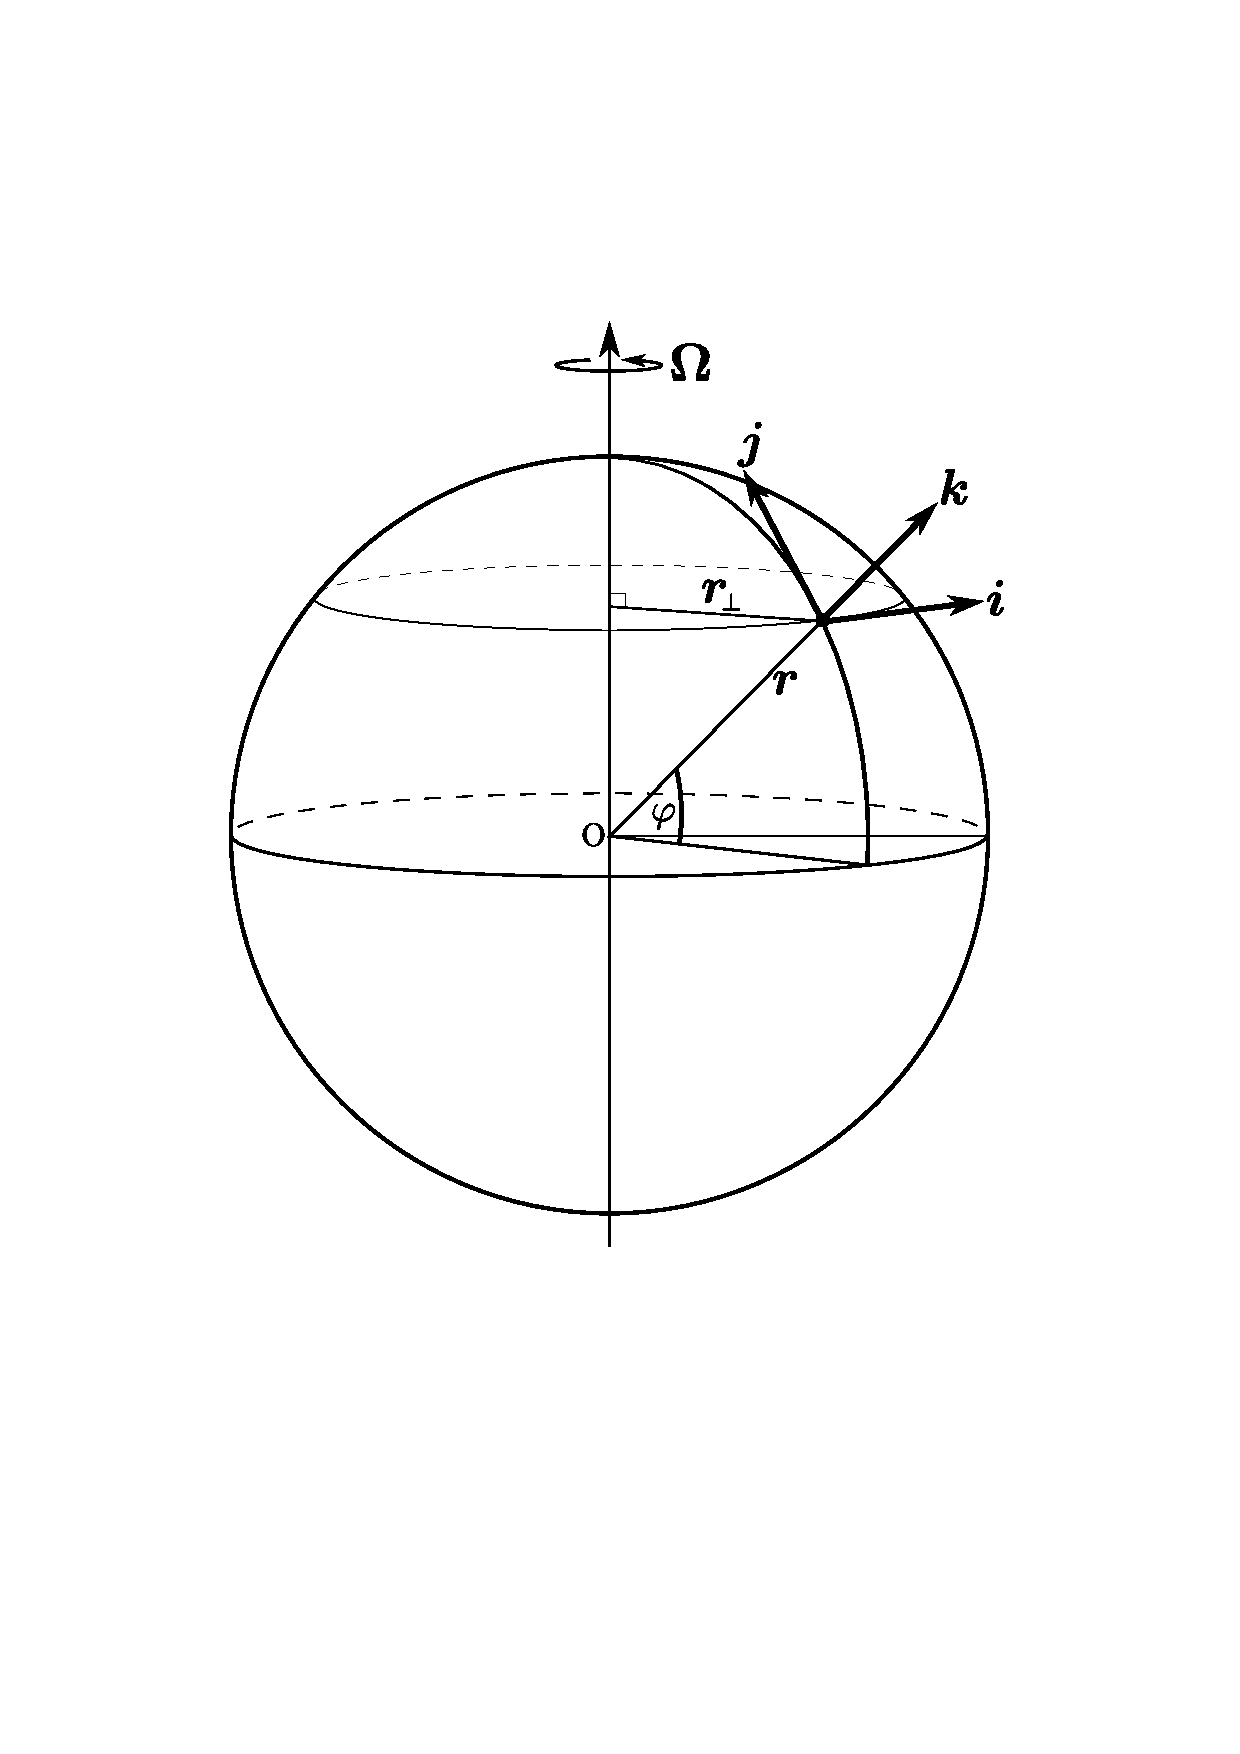
\includegraphics[width=8.0cm]{misc_images/coordinates.pdf}
\caption{Schematic of coordinates in a frame rotating with a sphere. The rotation is about a vector
pointing from South to North pole. A point on the surface of the sphere $\bmx$ and its perpendicular
distance from the axes of rotation $\bmx_{\perp}$ are shown. The latitude of $\bmx$ is given by $\phi$ 
and the unit vectors $\bmi$, $\bmj$ and $\bmk$ represent a local coordinate axes at point $\bmx$ in the rotating
frame: $\bmi$ points Eastwards, $\bmj$ points Northwards and $\bmk$ points in the radial outwards direction.}
\end{figure}

It is possible to form the equations with respect to a moving reference frame as long as the
additional force or acceleration term is included. In the case of a rotating frame that is
just by replacing the material derivative in the momentum equation by
\begin{equation}
\DDt{\bmu} + 2\bmOmega\times\bmu,
\end{equation}
where $\bmOmega$ is the angular velocity vector of the rotating
system.

Consider the Earth with a rotation vector in an inertial reference frame given by 
\begin{equation}\label{eq:on_sphere_rotation}
\bmOmega=(0,0,\Omega)^T.
\end{equation}
In a local rotating frame of reference where the
$x$-axis is oriented Eastwards,
the $y$-axis is oriented Northwards and the $z$-axis is the local upwards direction,
the Earth's rotation vector is expressed as
\begin{equation*}
\bmOmega = \Omega \cos \phi\; {\bf j} + \Omega \sin \phi\; {\bf k} \equiv \Omega (0,\cos\phi,\sin\phi)^T,
\end{equation*}
where $\phi$ is the latitude.
The acceleration terms in the three momentum equations now have the form
{\setlength\arraycolsep{2pt}
\begin{eqnarray*}
&&\DDt{u} {\color{red}+} {\color{red}2\Omega\cos\phi\; w} - 2\Omega\sin\phi\; v,\\
&&\DDt{v} + 2\Omega\sin\phi\; u,\\
&&\DDt{w} {\color{red}-} {\color{red}2\Omega\cos\phi\; v}.
\end{eqnarray*}}

\subsubsection{The `traditional' approximation}
\index{traditional approximation}
Define the Coriolis and reciprocal Coriolis parameters \citep{cushman1994} respectively by
\begin{equation}\label{eq:coriolis_parameters} 
f=2\Omega\sin\phi,\quad f^*=2\Omega\cos\phi.
\end{equation}
Due to dimensional considerations it is is usual to
drop the $f^*$ term and hence simply assume that 
\begin{equation}\label{eq:f_omega}
\bmOmega=(0,0,f/2)^T,
\end{equation}
in the local frame of reference, \ie only to consider the locally vertical
component of the rotation vector.
This approximation, when taken along with the assumption of hydrostatic balance in the
vertical constitutes what is generally known as the traditional approximation in geophysical fluid
dynamics.


\subsubsection{The $f$-plane and beta plane approximations}
\index{Coriolis!f-plane@$f$-plane}
\index{Coriolis!b-plane@$\beta$-plane}
If the Coriolis parameter $f$ is approximated by a constant value:
\begin{equation}\label{eq:f-plane}
f=f_0,
\end{equation}
this is termed the $f$-plane approximation, 
where $f_0 = 2\Omega\sin\phi_0$ at a latitude $\phi_0$.
This is obviously only an applicable approximation in a domain of interest 
that does not have large extent in latitude. 

For slightly larger domains a more accurate approximation is to use
\begin{equation}\label{eq:beta-plane}
f = f_0 + \beta y,
\end{equation}
where $y$ is the local coordinate in the Northwards direction.
Taking $\phi = \phi_0 + y/R_E$ and expanding \eqref{eq:coriolis_parameters} 
in a Taylor series yields
\begin{equation*}
f = f_0 +2\Omega\cos\phi_0\frac{y}{R_E}+\ldots,\quad \beta = \frac{2\Omega}{R_E}\cos\phi_0,
\end{equation*}
where $R_E\approx\unit[6378]{km}$. Typical values of these terms are: 
\begin{equation*}
\Omega = \frac{2\pi}{24\times 60\times 60} = 7.2722\times 10^{-5}\rads[],
\end{equation*}
(NB. a sidereal day should be used to give a more accurate value of $7.2921\times 10^{-5}\rads[]$)
and
\begin{center}\begin{small}
\begin{tabular}{c|ccc}
  &  $\phi_0 = 30$ & $\phi_0=45$ & $\phi_0 = 60$ \\  \hline
 $f_0$  & 7.2722e-05 & 1.0284e-04 & 1.2596e-04 \\
 $\beta$  & 1.9750e-11  &  1.6124e-11  &  1.1402e-11 \\
\end{tabular}\end{small}
\end{center}


\subsection{Multi-material Simulations}
\index{multi-material flow}
The ability to differentiate between regions with distinct material properties is of fundamental importance in the modelling of many physical systems.  Two different approaches exist for achieving this: the multi-material approach and the multi-phase approach.  The Multi-material approach is currently implemented within \fluidity. Multi-phase is currently under development and is therefore not discussed here. 
In situations where the model can resolve physical mixing of immiscible materials, or where there is no mixing, only one velocity field (and hence one momentum equation) is required to describe the flow of all materials. The \emph{multi-material} approach, considers all materials to be immiscible materials separated by a sharp interface.

In a multi-material approach, the various forms of the conservation equations can be solved for multiple material flows if the pointwise mass density $\rho$ in the equations is defined as the bulk density at each point.  If the flow comprises $n$ materials and the volume fraction of the $i^{th}$ material is denoted $\phi_i$ then the bulk density is given by:
\begin{equation}
\rho = \sum_{i=1}^n \phi_i\rho_i
\end{equation}
where $\rho_i$ is the density of each material.  For incompressible materials $\rho_i = \rho_{i0}$; for materials whose density is defined by an equation of state (see section~\ref{sect:equation_of_state}) $\rho_i = f(p,T,S,\ldots)$.  Conservation of mass at each point also requires that
\begin{equation}
\sum_{i=1}^n \phi_{i} = 1.
\end{equation}

In an $n$-material problem, the multi-material approach requires that $n-1$ advection equations are solved, to describe the transport of the volume fraction of all but one of the materials.  The volume fraction of the remaining material can be derived from the other volume fractions by
\begin{equation}\label{diagnosticvolfrac}
\phi_{n} = 1 - \sum_{i=1}^{n-1}\phi_{i}. 
\end{equation}
The transport of the $i^{th}$ volume fraction is given by  
\begin{equation}
\ppt{\phi_i} + \bmu\cdot\nabla\phi_i = 0,
\end{equation}
where the volume fraction field at time zero must be specified.


\subsection{Absorption, Reaction and Source Terms}
The absorption term in \eqref{eq:general_scalar_eqn} 
\begin{equation}\label{eq:scalar_absorption}
-\sigma c,
\end{equation}
has the effect of decreasing the magnitude of $c$ (note the minus sign and the fact 
that $\sigma$ would typically be positive. It is sometimes termed Rayleigh friction. 

The remaining term in \eqref{eq:general_scalar_eqn}
\begin{equation}\label{eq:scalar_source}
F = \sum_i F_i,
\end{equation}
can encompasses a number of source and reaction terms. Those terms where $F_i$ are
a given function of time, location or a-priori known fields are termed sources (and sometime
sinks if they are negative). Those terms which are also functions of other prognostic fields
are termed reactions and are common when dealing with chemistry or biology.

\subsection{Free surface}\label{Sect:FS}
\index{free surface}
The free surface height $\eta\equiv\eta(x,y,t)$ measured from the initial state of the ocean
may be modelled either via the integrated continuity equation,
or for simplicity here by the kinematic boundary condition which simply states
that particles on the free surface remain on it, \ie
\begin{equation}\label{freesurf2}
\frac{\partial \eta}{\partial t}=-\left.{\bmu}_H\right|_{z=\eta}\cdot\nabla_H \eta +\left.w\right|_{z=\eta} \quad \textrm{on}\quad \Gamma_{FS},
\end{equation}
where $\Omega_{FS}\subset \partial \Omega$ is the free surface boundary, $\nabla_H\equiv(\partial/\partial x,\partial/\partial y)^T$, and
$\bmu_H$ is the horizontal component of $\bmu$. Using the fact that the normal vector $\vec n$ at the free surface is $\frac{(-\frac{\partial \eta}{\partial x},-\frac{\partial \eta}{\partial y}, 1)^T}{||(-\frac{\partial \eta}{\partial x},-\frac{\partial \eta}{\partial y}, 1)^T||}$, equation \eqref{freesurf2} can be reformulated to
\begin{equation}\label{freesurf3}
\frac{\partial \eta}{\partial t}=\frac{\bmu \cdot \vec n}{\vec n \cdot \vec z},
\end{equation}
where $\vec z=(0,0,1)$ is the vertical standard basis vector.
